

\section{Finding Peaks} \label{FindPeaks}
	To generalize the procedure of peak characterization we need to be able to detect all the peaks in the data set and study them. To do this, we follow the procedure described in  \cite{DetectPeaks}. We use a simplified form of this algorithm, adapted to our needs and the present data set.
	The way our algorithm works is by declaring all the points in the data set as a possible peak and then start removing peaks that do not satisfy some criteria, namely:
	\begin{enumerate}
  	\item Promote all the data points to peak candidates;
	 \item Remove all the points that are below a certain threshold (defined by the user) - mph;
	 \item Remove all the points that are close to a higher peak, where the distance is defined by the user - mpd;	 
	\end{enumerate}

	Once we detect all the peaks in a data set, we can use the algorithm defined in the previous section (gaussian fit) to construct a list with all the peaks and their variables (number of peaks, areas, centers and widths).
	Figure \ref{fig:findpeaks} shows the detected peaks in the intensity profile for T = 0 K. Ideally we would have systematically tried different values of thresholds for height and distance as described in the algorithm. But in this first study we simply used reasonable values without optimization. A complete optimization of these hyper-parameters is necessary to improve results. But as discussed before, drastic changes in the material structure will still be detected even without further optimization.
	To find the height threshold we first calculate the average intensity of the data set and the standard deviation. We define the threshold as:
	\begin{equation} \label{eq:mph}
	mph = \mu + 1.5\cdot \sigma,
	\end{equation}
	where $\mu$ is the mean value of the data set and $\sigma$, the standard deviation. For the minimum distance we used mpd = 50, i.e, tow peaks have to be at least 50 points apart in the data set.
	
\begin{figure}[h]
  \centering
  %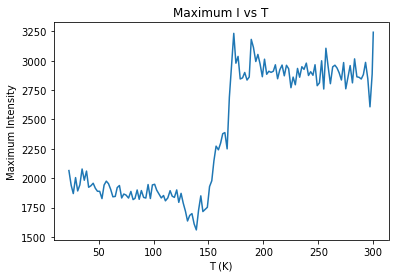
\includegraphics[scale=0.1, width=0.8\linewidth]{../figs/maxI.png}
  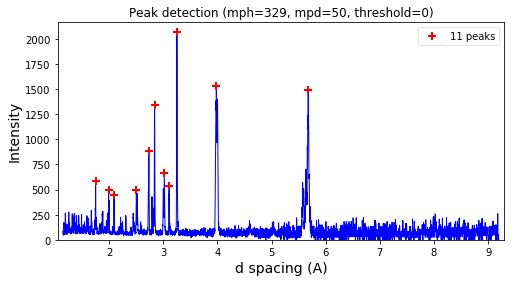
\includegraphics[scale=0.25]{../figs/peaks0.png}
  \caption{Intensity as a function of d-spacing for T = 0 K. The red points indicate the detected peaks in the data.}
  \label{fig:findpeaks}
\end{figure}